% MutBench PhD Dissertation Defense Presentation
% Compile with: xelatex presentation.tex
\PassOptionsToPackage{table}{xcolor}
\documentclass[aspectratio=169,11pt]{beamer}

\usetheme{Madrid}
\usecolortheme{default}

% ── Packages ──
\usepackage{fontspec}
\setmainfont{TeX Gyre Termes}
\usepackage{booktabs}
\usepackage{tikz}
\usetikzlibrary{arrows.meta, positioning, shapes.geometric, calc, fit}
\usepackage{adjustbox}
\usepackage{array}
\usepackage{multirow}
\usepackage{amsmath}
% xcolor with table option loaded via \PassOptionsToPackage before \documentclass

% ── Color definitions ──
\definecolor{stage1blue}{RGB}{31,119,180}
\definecolor{stage2orange}{RGB}{255,127,14}
\definecolor{pahdgreen}{RGB}{44,160,44}
\definecolor{lightgray}{RGB}{240,240,240}
\definecolor{darktext}{RGB}{50,50,50}
\definecolor{alertred}{RGB}{214,39,40}

% ── Beamer customization ──
\setbeamercolor{structure}{fg=stage1blue}
\setbeamercolor{frametitle}{bg=stage1blue!10, fg=stage1blue!90!black}
\setbeamercolor{title}{fg=white, bg=stage1blue}
\setbeamercolor{block title}{bg=stage1blue, fg=white}
\setbeamercolor{block body}{bg=stage1blue!5}
\setbeamercolor{alerted text}{fg=alertred}
\setbeamerfont{frametitle}{series=\bfseries}
\setbeamertemplate{navigation symbols}{}
\setbeamertemplate{footline}{%
  \leavevmode\hbox{%
    \begin{beamercolorbox}[wd=.33\paperwidth,ht=2.5ex,dp=1ex,center]{author in head/foot}%
      \usebeamerfont{author in head/foot}\insertshortauthor
    \end{beamercolorbox}%
    \begin{beamercolorbox}[wd=.34\paperwidth,ht=2.5ex,dp=1ex,center]{title in head/foot}%
      \usebeamerfont{title in head/foot}\insertshorttitle
    \end{beamercolorbox}%
    \begin{beamercolorbox}[wd=.33\paperwidth,ht=2.5ex,dp=1ex,right]{date in head/foot}%
      \usebeamerfont{date in head/foot}\insertframenumber{} / \inserttotalframenumber\hspace*{2ex}
    \end{beamercolorbox}}%
}

% ── Title info ──
\title[MutBench]{MutBench: Systematic Benchmarking for\\Viral Mutation Hotspot Detection}
\author[H. Kwon]{Hwijun Kwon\\[0.5em]{\small Advisor: Prof.\ Inuk Jung}}
\institute[KNU]{School of Computer Science and Engineering\\Kyungpook National University}
\date{August 2026}

\begin{document}

% ════════════════════════════════════════════════════════════
% SLIDE 1: TITLE
% ════════════════════════════════════════════════════════════
\begin{frame}[plain]
\titlepage
\end{frame}

% ════════════════════════════════════════════════════════════
% SLIDE 2: WHAT ARE MUTATION HOTSPOTS?
% ════════════════════════════════════════════════════════════
\begin{frame}{Mutation Hotspots Drive Viral Evolution}

\begin{columns}[T]
\begin{column}{0.55\textwidth}
\textbf{Definition:} Genomic positions with elevated mutation rates compared to background

\vspace{1em}
\textbf{Why it matters:}
\begin{itemize}
  \item Vaccine target prioritization
  \item Variant surveillance and early warning
  \item Drug resistance prediction
\end{itemize}

\vspace{1em}
\textbf{Examples (SARS-CoV-2 Spike):}\\
N501Y, E484K, L452R --- all at known hotspots
\end{column}

\begin{column}{0.42\textwidth}
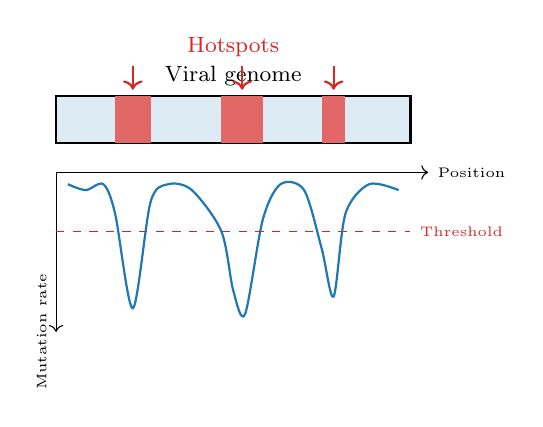
\begin{tikzpicture}[scale=0.75, every node/.style={font=\small}]
  % Genome bar
  \fill[stage1blue!15] (0,0) rectangle (6,0.8);
  \draw[thick] (0,0) rectangle (6,0.8);
  \node[above] at (3,0.8) {\footnotesize Viral genome};
  % Hotspot regions
  \fill[alertred!70] (1.0,0) rectangle (1.6,0.8);
  \fill[alertred!70] (2.8,0) rectangle (3.5,0.8);
  \fill[alertred!70] (4.5,0) rectangle (4.9,0.8);
  % Labels
  \draw[->, thick, alertred] (1.3,1.3) -- (1.3,0.9);
  \draw[->, thick, alertred] (3.15,1.3) -- (3.15,0.9);
  \draw[->, thick, alertred] (4.7,1.3) -- (4.7,0.9);
  \node[alertred, above] at (3.0,1.3) {\footnotesize Hotspots};
  % Mutation rate plot
  \draw[->] (0,-0.5) -- (6.3,-0.5) node[right] {\tiny Position};
  \draw[->] (0,-0.5) -- (0,-3.2) node[left, rotate=90, anchor=south] {\tiny Mutation rate};
  % Simulated rate curve
  \draw[stage1blue, thick] plot[smooth] coordinates {
    (0.2,-0.7) (0.5,-0.8) (0.8,-0.7) (1.0,-1.2) (1.3,-2.8) (1.6,-1.0) (1.9,-0.7)
    (2.3,-0.8) (2.8,-1.5) (3.0,-2.5) (3.2,-2.9) (3.5,-1.3) (3.8,-0.7)
    (4.2,-0.8) (4.5,-1.8) (4.7,-2.6) (4.9,-1.2) (5.3,-0.7) (5.8,-0.8)
  };
  % Threshold line
  \draw[dashed, alertred] (0,-1.5) -- (6,-1.5) node[right] {\tiny Threshold};
\end{tikzpicture}
\end{column}
\end{columns}
\end{frame}

% ════════════════════════════════════════════════════════════
% SLIDE 3: THE PROBLEM — NO BENCHMARK EXISTS
% ════════════════════════════════════════════════════════════
\begin{frame}{No Systematic Benchmark Exists for Hotspot Detection}

\begin{center}
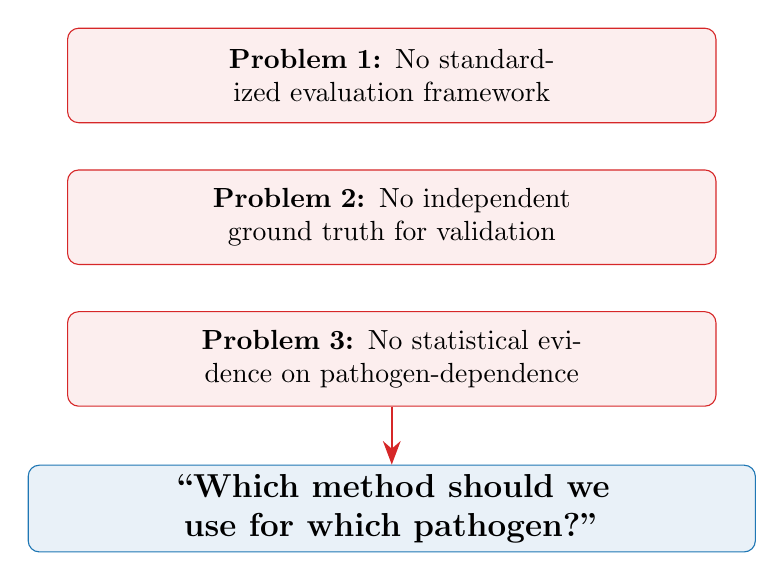
\begin{tikzpicture}[
  problem/.style={draw=alertred, fill=alertred!8, rounded corners, text width=8cm,
    minimum height=1.2cm, align=center, font=\normalsize},
  arrow/.style={-{Stealth[length=3mm]}, thick, alertred}
]
  \node[problem] (p1) at (0, 2.0) {\textbf{Problem 1:} No standardized evaluation framework};
  \node[problem] (p2) at (0, 0.2) {\textbf{Problem 2:} No independent ground truth for validation};
  \node[problem] (p3) at (0,-1.6) {\textbf{Problem 3:} No statistical evidence on pathogen-dependence};
  \node[draw=stage1blue, fill=stage1blue!10, rounded corners, text width=9cm,
    minimum height=1.0cm, align=center, font=\large\bfseries] (q) at (0,-3.5)
    {``Which method should we use for which pathogen?''};
  \draw[arrow] (p3.south) -- (q.north);
\end{tikzpicture}
\end{center}
\end{frame}

% ════════════════════════════════════════════════════════════
% SLIDE 4: RESEARCH CONTRIBUTIONS
% ════════════════════════════════════════════════════════════
\begin{frame}{Two Contributions: Framework + Statistical Evidence}

\begin{columns}[T]
\begin{column}{0.48\textwidth}
\begin{block}{\textcolor{stage1blue}{Contribution 1: MutBench Framework}}
\begin{itemize}
  \item 3-layer ground truth\\(convergent / purifying / DMS)
  \item Hotspot-score composite metric
  \item 2-stage experimental design\\(depth-first + breadth-first)
\end{itemize}
\end{block}
\end{column}

\begin{column}{0.48\textwidth}
\begin{block}{\textcolor{stage2orange}{Contribution 2: Statistical Demonstration}}
\begin{itemize}
  \item Interaction $\omega^2 = $ \alert{0.285}\\(largest variance source)
  \item LOPO: \alert{0/9} generalization
  \item Friedman: $p = $ \alert{0.0015}
  \item 9/9 unique best combinations
\end{itemize}
\end{block}
\end{column}
\end{columns}

\vspace{1em}
\begin{center}
\colorbox{pahdgreen!10}{\parbox{0.85\textwidth}{\centering
\textcolor{pahdgreen}{\textbf{Implication:}} No universal best method $\to$ pathogen-adaptive selection is essential
}}
\end{center}
\end{frame}

% ════════════════════════════════════════════════════════════
% SLIDE 5: MUTBENCH PIPELINE OVERVIEW
% ════════════════════════════════════════════════════════════
\begin{frame}{MutBench: End-to-End Benchmark Pipeline}

\begin{center}
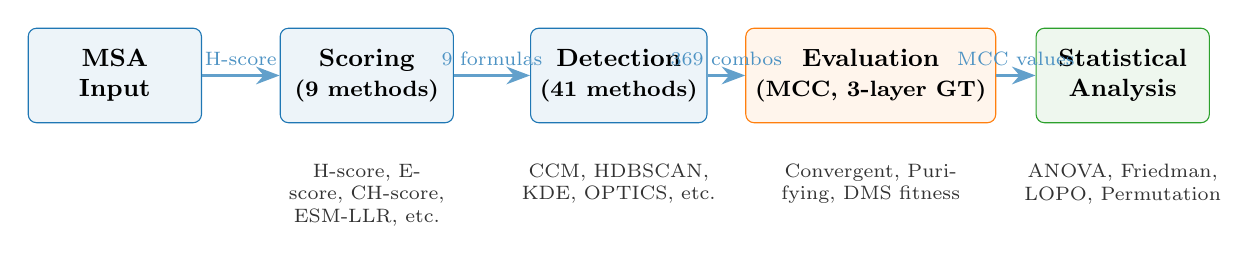
\begin{tikzpicture}[
  box/.style={draw=stage1blue, fill=stage1blue!8, rounded corners=3pt,
    minimum width=2.2cm, minimum height=1.2cm, align=center, font=\small\bfseries},
  arr/.style={-{Stealth[length=3mm]}, thick, stage1blue!70},
  lbl/.style={font=\scriptsize, stage1blue!80, above, midway}
]
  \node[box] (msa) at (0,0) {MSA\\Input};
  \node[box] (score) at (3.2,0) {Scoring\\{\footnotesize (9 methods)}};
  \node[box] (detect) at (6.4,0) {Detection\\{\footnotesize (41 methods)}};
  \node[box, draw=stage2orange, fill=stage2orange!8] (eval) at (9.6,0) {Evaluation\\{\footnotesize (MCC, 3-layer GT)}};
  \node[box, draw=pahdgreen, fill=pahdgreen!8] (stat) at (12.8,0) {Statistical\\Analysis};

  \draw[arr] (msa) -- (score) node[lbl] {H-score};
  \draw[arr] (score) -- (detect) node[lbl] {9 formulas};
  \draw[arr] (detect) -- (eval) node[lbl] {369 combos};
  \draw[arr] (eval) -- (stat) node[lbl] {MCC values};

  % Bottom annotations
  \node[font=\scriptsize, darktext, below=0.4cm, text width=2.5cm, align=center] at (score.south) {H-score, E-score, CH-score, ESM-LLR, etc.};
  \node[font=\scriptsize, darktext, below=0.4cm, text width=2.5cm, align=center] at (detect.south) {CCM, HDBSCAN, KDE, OPTICS, etc.};
  \node[font=\scriptsize, darktext, below=0.4cm, text width=2.5cm, align=center] at (eval.south) {Convergent, Purifying, DMS fitness};
  \node[font=\scriptsize, darktext, below=0.4cm, text width=2.5cm, align=center] at (stat.south) {ANOVA, Friedman, LOPO, Permutation};
\end{tikzpicture}
\end{center}

\vspace{0.5em}
\begin{center}
{\footnotesize \textcolor{stage1blue}{Stage 1:} SARS-CoV-2 depth-first (5 variants + 2 baselines) \quad
\textcolor{stage2orange}{Stage 2:} 9 pathogens breadth-first (3,321 evaluations)}
\end{center}
\end{frame}

% ════════════════════════════════════════════════════════════
% SLIDE 6: 3-LAYER GROUND TRUTH
% ════════════════════════════════════════════════════════════
\begin{frame}{Three Independent Ground Truth Layers Ensure Robust Evaluation}

\begin{center}
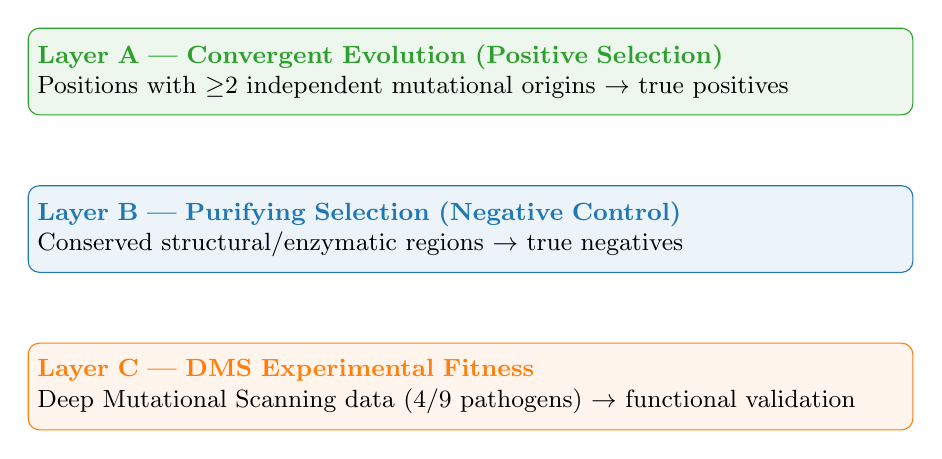
\begin{tikzpicture}[
  layer/.style={draw=#1, fill=#1!8, rounded corners, text width=11cm,
    minimum height=1.1cm, align=left, font=\small},
]
  \node[layer=pahdgreen] (la) at (0, 2.0) {
    \textbf{\textcolor{pahdgreen}{Layer A --- Convergent Evolution (Positive Selection)}}\\
    Positions with $\geq$2 independent mutational origins $\to$ true positives
  };
  \node[layer=stage1blue] (lb) at (0, 0.0) {
    \textbf{\textcolor{stage1blue}{Layer B --- Purifying Selection (Negative Control)}}\\
    Conserved structural/enzymatic regions $\to$ true negatives
  };
  \node[layer=stage2orange] (lc) at (0,-2.0) {
    \textbf{\textcolor{stage2orange}{Layer C --- DMS Experimental Fitness}}\\
    Deep Mutational Scanning data (4/9 pathogens) $\to$ functional validation
  };
\end{tikzpicture}
\end{center}

\vspace{0.5em}
\begin{center}
\textbf{Independence:} Jaccard(DMS, convergent) = \alert{0.006}\\[0.3em]
{\footnotesize The three layers capture different biological signals, preventing circular validation.}
\end{center}
\end{frame}

% ════════════════════════════════════════════════════════════
% SLIDE 7: HOTSPOT-SCORE METRIC
% ════════════════════════════════════════════════════════════
\begin{frame}{Hotspot-Score: A Composite Metric Beyond F1}

\begin{center}
\Large
$\text{hotspot-score} = \dfrac{\text{recall} + \text{precision} + \text{stability}}{3}$
\end{center}

\vspace{0.5em}
\textbf{Why not F1 alone?}

\begin{center}
\begin{tabular}{lcccc}
\toprule
\textbf{Method} & \textbf{Recall} & \textbf{Precision} & \textbf{Stability} & \textbf{HS} \\
\midrule
\textbf{MutClust-Hybrid} & 0.659 & \textbf{0.968} & 0.706 & \textbf{0.778} \\
HDBSCAN-Auto & \textbf{0.944} & 0.079 & 0.788 & 0.604 \\
\bottomrule
\end{tabular}
\end{center}

\vspace{0.5em}
\begin{itemize}
  \item HDBSCAN detects \alert{14,916} positions (half the genome) --- high recall, low precision
  \item F1 misses the stability dimension (robustness to input perturbation)
  \item Hotspot-score correctly identifies Hybrid as best (\alert{0.778} vs.\ 0.604)
\end{itemize}
\end{frame}

% ════════════════════════════════════════════════════════════
% SLIDE 8: TWO-STAGE EXPERIMENTAL DESIGN
% ════════════════════════════════════════════════════════════
\begin{frame}{Two-Stage Design: Depth-First Then Breadth-First}

\begin{center}
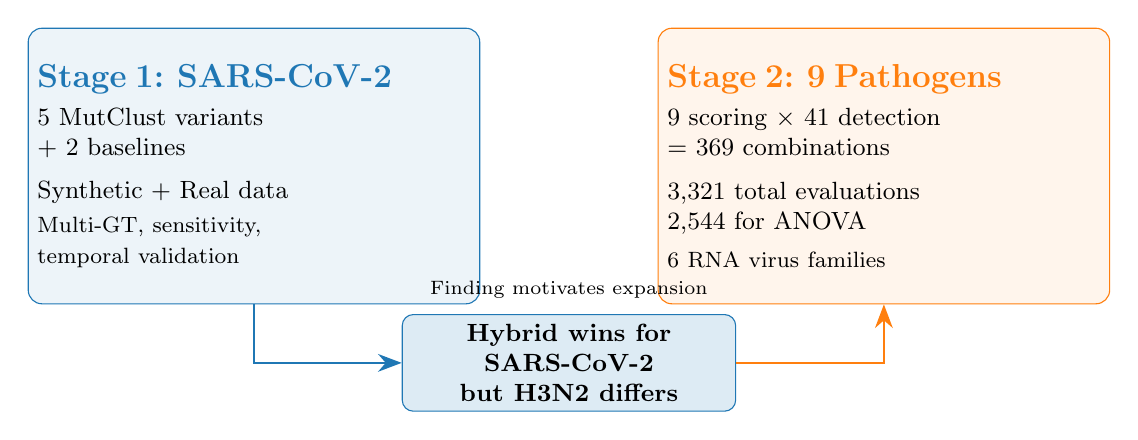
\begin{tikzpicture}[
  stage/.style={draw=#1, fill=#1!8, rounded corners=5pt, text width=5.5cm,
    minimum height=3.5cm, align=left, font=\small},
  finding/.style={draw=#1, fill=#1!15, rounded corners, font=\small\bfseries,
    text width=4cm, align=center}
]
  % Stage 1
  \node[stage=stage1blue] (s1) at (-4,0) {
    \textbf{\textcolor{stage1blue}{\large Stage 1: SARS-CoV-2}}\\[0.3em]
    5 MutClust variants\\+ 2 baselines\\[0.5em]
    Synthetic + Real data\\[0.3em]
    {\footnotesize Multi-GT, sensitivity,\\temporal validation}
  };

  % Stage 2
  \node[stage=stage2orange] (s2) at (4,0) {
    \textbf{\textcolor{stage2orange}{\large Stage 2: 9 Pathogens}}\\[0.3em]
    9 scoring $\times$ 41 detection\\= 369 combinations\\[0.5em]
    \alert{3,321} total evaluations\\
    \alert{2,544} for ANOVA\\[0.3em]
    {\footnotesize 6 RNA virus families}
  };

  % Arrow
  \node[finding=stage1blue] (f1) at (0,-2.5) {Hybrid wins for SARS-CoV-2\\but H3N2 differs};
  \draw[-{Stealth[length=3mm]}, thick, stage1blue] (s1.south) |- (f1.west);
  \draw[-{Stealth[length=3mm]}, thick, stage2orange] (f1.east) -| (s2.south);
  \node[font=\scriptsize, above] at (0,-1.8) {Finding motivates expansion};
\end{tikzpicture}
\end{center}
\end{frame}

% ════════════════════════════════════════════════════════════
% SLIDE 9: STAGE 1 — MUTCLUST-HYBRID IS BEST (SARS-CoV-2)
% ════════════════════════════════════════════════════════════
\begin{frame}{\textcolor{stage1blue}{Stage 1:} MutClust-Hybrid Achieves Best Hotspot-Score}

\begin{center}
\begin{tabular}{lcccc}
\toprule
\textbf{Method} & \textbf{Precision} & \textbf{Recall} & \textbf{Stability} & \textbf{HS} \\
\midrule
\rowcolor{pahdgreen!12}
\textbf{MutClust-Hybrid} & \textbf{0.968} & \textbf{0.659} & \textbf{0.706} & \textbf{0.778} \\
MutClust-Fixed & 0.988 & 0.506 & 0.445 & 0.646 \\
MutClust-Original & 0.991 & 0.504 & 0.418 & 0.638 \\
HDBSCAN-Auto & 0.079 & 0.944 & 0.788 & 0.604 \\
\midrule
Two-stage intersection & 0.968 & 0.643 & 0.740 & 0.784 \\
\bottomrule
\end{tabular}
\end{center}

\vspace{0.5em}
\begin{itemize}
  \item CCM seed detection $+$ HDBSCAN boundary $\to$ best of both worlds
  \item Hybrid ranking robust in \alert{71.9\%} of 171 weight combinations
  \item Two-stage intersection achieves highest HS (0.784) with improved stability
\end{itemize}
\end{frame}

% ════════════════════════════════════════════════════════════
% SLIDE 10: REAL DATA TELLS A DIFFERENT STORY
% ════════════════════════════════════════════════════════════
\begin{frame}{Synthetic Success Does Not Transfer Directly to Real Data}

\begin{columns}[T]
\begin{column}{0.48\textwidth}
\textbf{Performance gap:}
\begin{center}
\begin{tabular}{lcc}
\toprule
& \textbf{Synth.} & \textbf{Real} \\
\midrule
F1 & 0.785 & \alert{0.123} \\
Enrichment & 23.2$\times$ & 7.3$\times$ \\
\bottomrule
\end{tabular}
\end{center}

\vspace{0.5em}
F1 drops by \alert{0.66}, but enrichment ratios remain consistently high at \textbf{6.9--8.0$\times$}.
\end{column}

\begin{column}{0.48\textwidth}
\textbf{H-score saturation:}
\begin{itemize}
  \item Real GISAID data: only 342 of 29,903 positions are nonzero
  \item Sparse distribution $\to$ low absolute recall
  \item Enrichment ratio confirms biological validity despite low F1
\end{itemize}

\vspace{0.5em}
\textbf{Implication:}\\
Absolute metrics require careful interpretation; relative enrichment is more robust.
\end{column}
\end{columns}
\end{frame}

% ════════════════════════════════════════════════════════════
% SLIDE 11: H3N2 REVERSES THE RANKINGS
% ════════════════════════════════════════════════════════════
\begin{frame}{H3N2 Reverses Method Rankings --- Pathogen Matters}

\begin{center}
\begin{tabular}{lccc}
\toprule
\textbf{Method} & \textbf{Strategy} & \textbf{SARS-CoV-2 HS} & \textbf{H3N2 HS} \\
\midrule
MutClust-Fixed & CCM & 0.646 & \textbf{0.661} \\
\rowcolor{stage1blue!8}
MutClust-Hybrid & CCM+HDBSCAN & \textbf{0.778} & 0.577 \\
MutClust-Original & CCM & 0.638 & 0.572 \\
HDBSCAN-Auto & HDBSCAN & 0.604 & 0.490 \\
\bottomrule
\end{tabular}
\end{center}

\vspace{1em}
\begin{center}
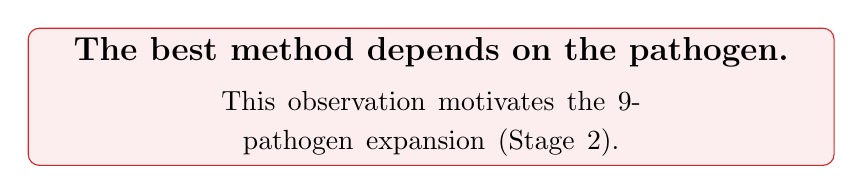
\begin{tikzpicture}
  \node[draw=alertred, fill=alertred!8, rounded corners, text width=10cm,
    align=center, font=\large\bfseries] {
    The best method depends on the pathogen.\\[0.3em]
    {\normalsize\normalfont This observation motivates the 9-pathogen expansion (Stage 2).}
  };
\end{tikzpicture}
\end{center}
\end{frame}

% ════════════════════════════════════════════════════════════
% SLIDE 12: STAGE 2 — 9 PATHOGENS
% ════════════════════════════════════════════════════════════
\begin{frame}{\textcolor{stage2orange}{Stage 2:} 9 Pathogens, 6 Virus Families, 3,321 Evaluations}

\begin{columns}[T]
\begin{column}{0.45\textwidth}
\textbf{Scale:}
\begin{itemize}
  \item 9 scoring formulas
  \item 41 detection methods (15 families)
  \item 9 RNA viruses
  \item \alert{3,321} total evaluations
  \item \alert{2,544} valid for ANOVA
\end{itemize}
\end{column}

\begin{column}{0.52\textwidth}
\textbf{Pathogen coverage:}\\[0.3em]
\footnotesize
\begin{tabular}{ll}
\toprule
\textbf{Family} & \textbf{Pathogens} \\
\midrule
Coronaviridae & SARS-CoV-2, MERS \\
Orthomyxoviridae & Influenza A (H3N2), Flu B \\
Retroviridae & HIV-1 \\
Pneumoviridae & RSV \\
Flaviviridae & Dengue, HCV \\
Caliciviridae & Norovirus \\
\bottomrule
\end{tabular}
\end{column}
\end{columns}

\vspace{0.5em}
\begin{center}
{\footnotesize Each pathogen evaluated with 3-layer ground truth (Layer C for 4 pathogens with DMS data)}
\end{center}
\end{frame}

% ════════════════════════════════════════════════════════════
% SLIDE 13: KEY FINDING — FOUR LINES OF EVIDENCE
% ════════════════════════════════════════════════════════════
\begin{frame}{No Universal Best Method: Four Independent Lines of Evidence}

\begin{center}
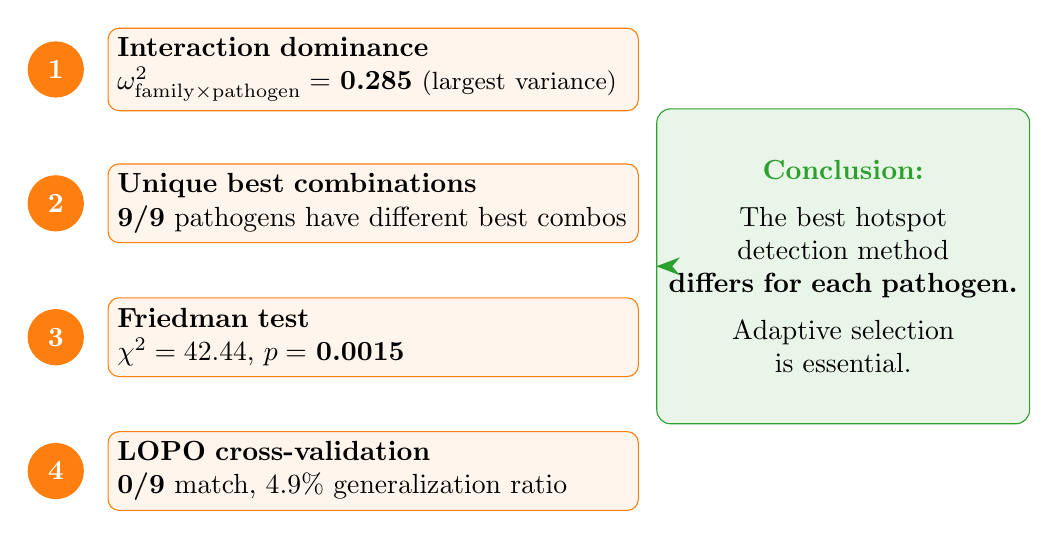
\begin{tikzpicture}[
  evidence/.style={draw=#1, fill=#1!8, rounded corners=4pt, text width=6.5cm,
    minimum height=1.0cm, align=left, font=\normalsize},
  num/.style={circle, draw=#1, fill=#1, text=white, font=\bfseries, minimum size=0.7cm}
]
  \node[num=stage2orange] (n1) at (-4.5, 2.5) {1};
  \node[evidence=stage2orange, right=0.3cm of n1] (e1) {
    \textbf{Interaction dominance}\\
    $\omega^2_{\text{family}\times\text{pathogen}} = $ \alert{\textbf{0.285}} {\small (largest variance)}
  };

  \node[num=stage2orange] (n2) at (-4.5, 0.8) {2};
  \node[evidence=stage2orange, right=0.3cm of n2] (e2) {
    \textbf{Unique best combinations}\\
    \alert{\textbf{9/9}} pathogens have different best combos
  };

  \node[num=stage2orange] (n3) at (-4.5,-0.9) {3};
  \node[evidence=stage2orange, right=0.3cm of n3] (e3) {
    \textbf{Friedman test}\\
    $\chi^2 = 42.44$, $p = $ \alert{\textbf{0.0015}}
  };

  \node[num=stage2orange] (n4) at (-4.5,-2.6) {4};
  \node[evidence=stage2orange, right=0.3cm of n4] (e4) {
    \textbf{LOPO cross-validation}\\
    \alert{\textbf{0/9}} match, 4.9\% generalization ratio
  };

  % Right side conclusion
  \node[draw=pahdgreen, fill=pahdgreen!10, rounded corners=5pt, text width=4.5cm,
    minimum height=4cm, align=center, font=\normalsize] (conc) at (5.5, 0) {
    \textbf{\textcolor{pahdgreen}{Conclusion:}}\\[0.5em]
    The best hotspot detection method\\
    \textbf{differs for each pathogen.}\\[0.5em]
    Adaptive selection\\is essential.
  };

  \draw[-{Stealth[length=3mm]}, thick, pahdgreen] (3.2, 0) -- (conc.west);
\end{tikzpicture}
\end{center}
\end{frame}

% ════════════════════════════════════════════════════════════
% SLIDE 14: ESM-2 CROSS-PARADIGM VALIDATION
% ════════════════════════════════════════════════════════════
\begin{frame}{Cross-Paradigm Validation: No Single Scoring Paradigm Dominates}

\textbf{ESM-2 (650M parameters):} MSA-free protein language model scoring

\begin{center}
\small
\begin{tabular}{lcccc}
\toprule
\textbf{Pathogen} & \textbf{ESM-LLR} & \textbf{Existing Best} & \textbf{$\Delta$} & \textbf{ESM Rank} \\
\midrule
\rowcolor{pahdgreen!12}
SARS-CoV-2 & 0.168 & 0.118 & +0.049 & \textbf{1/10} \\
\rowcolor{pahdgreen!12}
MERS & 0.143 & 0.088 & +0.055 & \textbf{1/10} \\
H3N2 & 0.360 & 0.549 & $-$0.189 & 5/10 \\
\rowcolor{alertred!8}
Norovirus & 0.176 & 0.438 & $-$0.262 & \textbf{10/10} \\
\rowcolor{alertred!8}
HIV-1 & 0.096 & 0.182 & $-$0.085 & \textbf{10/10} \\
\bottomrule
\end{tabular}
\end{center}

\vspace{0.5em}
\begin{itemize}
  \item ESM-LLR ranks \textcolor{pahdgreen}{\textbf{1st}} for SARS-CoV-2 and MERS, but \textcolor{alertred}{\textbf{last}} for Norovirus and HIV-1
  \item Reinforces: method--pathogen interaction dominates, even across paradigms
\end{itemize}
\end{frame}

% ════════════════════════════════════════════════════════════
% SLIDE 15: POSITION-EXACT IS CONSERVATIVE
% ════════════════════════════════════════════════════════════
\begin{frame}{Detected Hotspots Are Spatially Proximate to Ground Truth}

\textbf{Region-overlap MCC analysis} (relaxing exact position matching):

\begin{center}
\begin{tabular}{lccc}
\toprule
& \textbf{Exact} & \textbf{$\pm$5 nt} & \textbf{$\pm$10 nt} \\
\midrule
Mean MCC & 0.289 & 0.638 \textcolor{pahdgreen}{(+121\%)} & 0.712 \textcolor{pahdgreen}{(+146\%)} \\
H3N2 MCC & 0.521 & 0.964 & --- \\
\bottomrule
\end{tabular}
\end{center}

\vspace{1em}
\begin{itemize}
  \item Position-exact evaluation is \textbf{conservative}; off-by-one counts as FP
  \item Relaxing by $\pm$5 positions recovers substantial agreement
  \item Structural context: hotspot positions show \alert{5.92$\times$} spatial contact enrichment\\
        (within 8\AA{} distance, $z = 13.34$, $p < 0.001$)
\end{itemize}
\end{frame}

% ════════════════════════════════════════════════════════════
% SLIDE 16: PAHD — PROOF OF CONCEPT
% ════════════════════════════════════════════════════════════
\begin{frame}{\textcolor{pahdgreen}{PAHD:} Pathogen-Adaptive Hotspot Detection (Proof of Concept)}

\textbf{Problem:} 369 combinations, only $n = 9$ pathogens $\to$ exact prediction infeasible

\vspace{0.5em}
\textbf{Solution:} Predict at coarser granularity (family level, scoring level)

\begin{center}
\begin{tabular}{lcc}
\toprule
\textbf{Prediction level} & \textbf{Mean MCC} & \textbf{\% of Oracle} \\
\midrule
Exact combination & 0.005 & 1.7\% \\
Detection family (15) & 0.144 & 48.3\% \\
\rowcolor{pahdgreen!12}
\textbf{Scoring formula (9)} & \textbf{0.172} & \textbf{57.7\%} \\
\midrule
Oracle & 0.298 & 100\% \\
Naive LOPO & 0.021 & 8.2\% \\
\bottomrule
\end{tabular}
\end{center}

\vspace{0.3em}
\begin{itemize}
  \item v2 profile (85 MSA features) improves mean MCC from 0.005 to \alert{0.017}
  \item Critical bottleneck: $n = 9$ knowledge base $\to$ scaling to 20+ pathogens needed
\end{itemize}
\end{frame}

% ════════════════════════════════════════════════════════════
% SLIDE 17: PHYLOGENETIC CORRECTION — REAL DATA
% ════════════════════════════════════════════════════════════
\begin{frame}{Phylogenetic Correction: Founder Effects Confirmed}

\textbf{TreeTime ancestral reconstruction} on 500 SARS-CoV-2 sequences:

\vspace{0.5em}
\begin{columns}[T]
\begin{column}{0.48\textwidth}
\textbf{Key results:}
\begin{itemize}
  \item H-score vs.\ homoplasy: $\rho = -0.876$
  \item D614G: homoplasy = 0\\(founder effect confirmed)
  \item Real data MCC: $-0.018$\\(temporal mismatch)
\end{itemize}
\end{column}

\begin{column}{0.48\textwidth}
\textbf{Interpretation:}
\begin{itemize}
  \item High-frequency $\neq$ recurrently evolved
  \item 2020 early sequences predate VOC emergence
  \item Correction requires temporally aligned data
\end{itemize}
\end{column}
\end{columns}

\vspace{1em}
\begin{center}
\colorbox{stage2orange!10}{\parbox{0.8\textwidth}{\centering
\textbf{Limitation acknowledged:} Phylogenetic correction integration is Priority 1 for future work.
}}
\end{center}
\end{frame}

% ════════════════════════════════════════════════════════════
% SLIDE 18: LIMITATIONS & FUTURE ROADMAP
% ════════════════════════════════════════════════════════════
\begin{frame}{Limitations and Prioritized Future Research}

\begin{center}
\small
\begin{tabular}{llll}
\toprule
\textbf{Priority} & \textbf{Direction} & \textbf{Prerequisite} & \textbf{Expected Impact} \\
\midrule
\rowcolor{alertred!8}
1 (Highest) & Phylogenetic correction & TreeTime pipeline & Resolves founder-effect bias \\
\rowcolor{stage2orange!8}
2 & PAHD implementation & Corrected benchmark & Adaptive method selection \\
3 & DNA virus extension & New ground truth & Broader applicability \\
4 & Real-time surveillance & Incremental H-score & Public health utility \\
\bottomrule
\end{tabular}
\end{center}

\vspace{0.5em}
\textbf{Key limitations:}
\begin{itemize}
  \item DMS data available for 4/9 pathogens (remaining 5 use Layers A+B only)
  \item RNA viruses only; DNA virus mutation mechanisms differ
  \item $n = 9$ knowledge base insufficient for reliable PAHD combination prediction
\end{itemize}
\end{frame}

% ════════════════════════════════════════════════════════════
% SLIDE 19: CONCLUSIONS
% ════════════════════════════════════════════════════════════
\begin{frame}{Conclusions}

\begin{block}{\textcolor{stage1blue}{Contribution 1: MutBench Benchmark Framework}}
First systematic benchmark for viral mutation hotspot detection:\\
3-layer ground truth $+$ hotspot-score $+$ 2-stage design (3,321 evaluations across 9 pathogens)
\end{block}

\vspace{0.5em}

\begin{block}{\textcolor{stage2orange}{Contribution 2: Statistical Demonstration}}
No universal best method exists:
\begin{itemize}
  \item $\omega^2_{\text{family}\times\text{pathogen}} = 0.285$ (largest variance source)
  \item LOPO 0/9 $\cdot$ Friedman $p = 0.0015$ $\cdot$ 9/9 unique best combos
\end{itemize}
\end{block}

\vspace{0.5em}

\begin{center}
\colorbox{pahdgreen!10}{\parbox{0.85\textwidth}{\centering
\textbf{\textcolor{pahdgreen}{Broader lesson:}} Method--pathogen interaction dominates performance variance.\\
Adaptive selection, not a fixed method, is the path forward.
}}
\end{center}
\end{frame}

% ════════════════════════════════════════════════════════════
% SLIDE 20: THANK YOU
% ════════════════════════════════════════════════════════════
\begin{frame}[plain]

\begin{center}
\vspace{2cm}
{\Huge\bfseries Thank You}

\vspace{1.5cm}
{\Large Questions?}

\vspace{1.5cm}
{\normalsize
\texttt{https://github.com/hwijun/mutbench}
}
\end{center}
\end{frame}


% ════════════════════════════════════════════════════════════
%                    BACKUP SLIDES
% ════════════════════════════════════════════════════════════
\appendix
\newcounter{framenumberappendix}
\setcounter{framenumberappendix}{\value{framenumber}}

\begin{frame}
\begin{center}
\vspace{2cm}
{\Huge\bfseries Backup Slides}
\vspace{1cm}
\end{center}
\end{frame}

% ════════════════════════════════════════════════════════════
% B1: ANOVA DIAGNOSTIC DETAILS
% ════════════════════════════════════════════════════════════
\begin{frame}{B1: ANOVA Diagnostic Tests Confirm Robustness}

\textbf{Assumption violations and mitigations:}

\vspace{0.5em}
\begin{tabular}{lll}
\toprule
\textbf{Test} & \textbf{Result} & \textbf{Mitigation} \\
\midrule
Shapiro-Wilk & $W = 0.971$, $p = 3.29 \times 10^{-22}$ & Mild non-normality \\
 & (skew = 0.12, kurtosis = 2.42) & ($n = 2{,}544$ ensures robustness) \\
Levene's test & Rejected for all factors & Large balanced design \\
\midrule
\multicolumn{3}{l}{\textbf{Non-parametric confirmation (Kruskal-Wallis):}} \\
\midrule
Pathogen & $H = 569.1$, $p < 10^{-117}$ & Confirms ANOVA \\
Detection family & $H = 86.1$, $p < 10^{-12}$ & Confirms ANOVA \\
Scoring & $H = 78.1$, $p < 10^{-13}$ & Confirms ANOVA \\
\bottomrule
\end{tabular}

\vspace{0.5em}
All ANOVA effects confirmed by non-parametric alternatives.
\end{frame}

% ════════════════════════════════════════════════════════════
% B2: FRIEDMAN TEST POWER
% ════════════════════════════════════════════════════════════
\begin{frame}{B2: Friedman Test --- Significant Across Multiple $k$ Values}

\textbf{Friedman test} with 9 pathogens as blocks:

\vspace{1em}
\begin{center}
\begin{tabular}{ccc}
\toprule
\textbf{Top-$k$ combos} & $\chi^2$ & $p$-value \\
\midrule
$k = 10$ & significant & $< 0.01$ \\
\rowcolor{stage2orange!12}
$k = 20$ & \textbf{42.44} & \textbf{0.0015} \\
$k = 30$ & significant & $< 0.01$ \\
$k = 50$ & significant & $< 0.01$ \\
\bottomrule
\end{tabular}
\end{center}

\vspace{1em}
Significant performance rank differences among top combinations persist regardless of the number of combinations included.
\end{frame}

% ════════════════════════════════════════════════════════════
% B3: PAHD v1 vs v2 DETAILED COMPARISON
% ════════════════════════════════════════════════════════════
\begin{frame}{B3: PAHD v1 vs.\ v2 Profile Comparison}

\small
\begin{center}
\begin{tabular}{lrrrr}
\toprule
\textbf{Pathogen} & \textbf{Oracle} & \textbf{Naive} & \textbf{PAHD v1} & \textbf{PAHD v2} \\
\midrule
Dengue      & 0.256 & 0.000 & $-$0.012 & $-$0.027 \\
H3N2        & 0.549 & 0.000 & 0.207 & 0.011 \\
HCV         & 0.443 & 0.000 & $-$0.291 & \textcolor{pahdgreen}{\textbf{0.141}} \\
HIV-1       & 0.182 & 0.000 & 0.014 & 0.014 \\
Influenza B & 0.361 & 0.000 & $-$0.190 & $-$0.027 \\
MERS        & 0.088 & 0.000 & $-$0.012 & $-$0.025 \\
Norovirus   & 0.438 & 0.192 & 0.217 & 0.118 \\
RSV         & 0.249 & 0.000 & 0.069 & $-$0.054 \\
SARS-CoV-2  & 0.118 & 0.000 & 0.045 & 0.000 \\
\midrule
Mean & 0.298 & 0.021 & 0.005 & \textbf{0.017} \\
Positive MCC & 9/9 & 1/9 & \textbf{5/9} & 4/9 \\
\bottomrule
\end{tabular}
\end{center}

\vspace{0.3em}
v2 (85 MSA features) reduces pathological negative transfers: HCV $-0.291 \to +0.141$.
\end{frame}

% ════════════════════════════════════════════════════════════
% B4: DMS THRESHOLD SENSITIVITY
% ════════════════════════════════════════════════════════════
\begin{frame}{B4: DMS Threshold Sensitivity (Layer C)}

\textbf{DMS fitness effect threshold} determines which positions are ``functionally important'':

\vspace{1em}
\begin{center}
\begin{tabular}{lcc}
\toprule
\textbf{Threshold} & \textbf{Layer C positions} & \textbf{Effect on GT size} \\
\midrule
$\leq -0.3$ (lenient) & More positions & Larger positive set \\
\rowcolor{stage1blue!8}
$\leq -0.5$ (default) & Moderate & Balanced \\
$\leq -0.7$ (strict) & Fewer positions & Smaller positive set \\
\bottomrule
\end{tabular}
\end{center}

\vspace{1em}
\begin{itemize}
  \item DMS measures in vitro molecular fitness (pseudovirus systems)
  \item May not fully capture in vivo fitness
  \item Available for 4/9 pathogens: SARS-CoV-2, H3N2, HIV-1, RSV
\end{itemize}
\end{frame}

% ════════════════════════════════════════════════════════════
% B5: MUTCLUST BUG DESCRIPTION
% ════════════════════════════════════════════════════════════
\begin{frame}{B5: MutClust Original Bug --- Diminishing Cluster Formula}

\textbf{Bug in original MutClust implementation:}

\vspace{1em}
\begin{itemize}
  \item CCM (Cluster of Central Mutations) detection uses an iterative growth formula
  \item Original code: cluster score \textbf{diminishes} as cluster grows\\
        (dividing by accumulated score instead of window score)
  \item Effect: artificially limits cluster boundary expansion
  \item Result: slightly fewer detected positions (637 vs.\ 641)
\end{itemize}

\vspace{1em}
\textbf{Impact:}
\begin{itemize}
  \item Hotspot-score difference is small: 0.638 (Original) vs.\ 0.646 (Fixed)
  \item Effect size $d \approx 0.15$ --- not detectable at $n = 7$ regions
  \item Bug fix alone does not change the fundamental ranking
\end{itemize}
\end{frame}

% ════════════════════════════════════════════════════════════
% B6: WEIGHT SENSITIVITY
% ════════════════════════════════════════════════════════════
\begin{frame}{B6: Hotspot-Score Weight Sensitivity (171 Combinations)}

\begin{columns}[T]
\begin{column}{0.48\textwidth}
\textbf{Weight space exploration:}\\
$w_r + w_p + w_s = 1$, step = 0.05

\vspace{0.5em}
\begin{itemize}
  \item \textbf{171} total combinations tested
  \item Hybrid ranks 1st in \alert{71.9\%} (123/171)
  \item HDBSCAN ranks 1st in 28.1\% (48/171)
\end{itemize}

\vspace{0.5em}
Rank switch occurs only when:\\
recall weight $\geq 0.60$ AND\\
precision weight $\leq 0.20$
\end{column}

\begin{column}{0.48\textwidth}
\small
\begin{tabular}{lcc}
\toprule
\textbf{Scenario} & \textbf{Best} & \textbf{HS} \\
\midrule
Equal (default) & Hybrid & 0.778 \\
Recall-oriented & Hybrid & 0.748 \\
Precision-oriented & Hybrid & 0.826 \\
Stability-oriented & Hybrid & 0.760 \\
\rowcolor{alertred!8}
Early warning & HDBSCAN & 0.740 \\
Vaccine design & Hybrid & 0.854 \\
Monitoring & Hybrid & 0.749 \\
\bottomrule
\end{tabular}
\end{column}
\end{columns}
\end{frame}

% ════════════════════════════════════════════════════════════
% B7: 9 PATHOGENS — 6 RNA VIRUS FAMILIES
% ════════════════════════════════════════════════════════════
\begin{frame}{B7: Nine Pathogens Spanning Six RNA Virus Families}

\begin{center}
\small
\begin{tabular}{llccl}
\toprule
\textbf{Family} & \textbf{Pathogen} & \textbf{Genome (kb)} & \textbf{DMS?} & \textbf{Best Scoring} \\
\midrule
\multirow{2}{*}{Coronaviridae} & SARS-CoV-2 & $\sim$30 & Yes & E*rare \\
 & MERS-CoV & $\sim$30 & No & rank(P*E) \\
\multirow{2}{*}{Orthomyxoviridae} & H3N2 & $\sim$13 & Yes & E\_only \\
 & Influenza B & $\sim$14 & No & H-score \\
Retroviridae & HIV-1 & $\sim$10 & Yes & E*rare \\
Pneumoviridae & RSV & $\sim$15 & Yes & P*E \\
\multirow{2}{*}{Flaviviridae} & Dengue & $\sim$11 & No & E*rare \\
 & HCV & $\sim$10 & No & E\_only \\
Caliciviridae & Norovirus & $\sim$8 & No & P*E*rare \\
\bottomrule
\end{tabular}
\end{center}

\vspace{0.5em}
No two pathogens share the same best scoring formula, further supporting the interaction finding.
\end{frame}

% ════════════════════════════════════════════════════════════
% B8: TREETIME PIPELINE
% ════════════════════════════════════════════════════════════
\begin{frame}{B8: TreeTime Phylogenetic Correction Pipeline}

\begin{center}
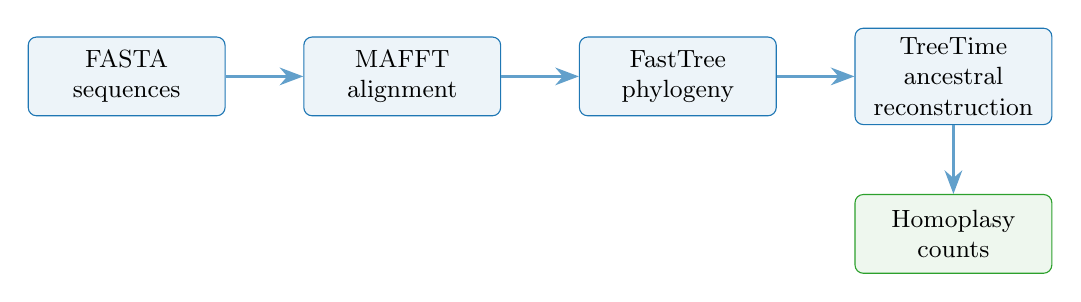
\begin{tikzpicture}[
  box/.style={draw=stage1blue, fill=stage1blue!8, rounded corners=3pt,
    minimum width=2.5cm, minimum height=1.0cm, align=center, font=\small},
  arr/.style={-{Stealth[length=3mm]}, thick, stage1blue!70}
]
  \node[box] (fasta) at (0,0) {FASTA\\sequences};
  \node[box] (align) at (3.5,0) {MAFFT\\alignment};
  \node[box] (tree) at (7,0) {FastTree\\phylogeny};
  \node[box] (tt) at (10.5,0) {TreeTime\\ancestral\\reconstruction};
  \node[box, draw=pahdgreen, fill=pahdgreen!8] (homo) at (10.5,-2) {Homoplasy\\counts};

  \draw[arr] (fasta) -- (align);
  \draw[arr] (align) -- (tree);
  \draw[arr] (tree) -- (tt);
  \draw[arr] (tt) -- (homo);
\end{tikzpicture}
\end{center}

\vspace{1em}
\textbf{Key results (simulation):}
\begin{itemize}
  \item AUC = 1.000 for TreeTime ML ancestral reconstruction ($N = 2{,}000$)
  \item $\rho = -0.876$ between H-score and independent mutational origins
  \item $\rho = -0.107$ on real GISAID sequences ($N = 500$)
  \item Computational bottleneck: TreeTime $O(N \log N)$; UShER enables millions of sequences
\end{itemize}
\end{frame}

% ════════════════════════════════════════════════════════════
% B9: MOSD → MUTBENCH DESIGN TRANSFER
% ════════════════════════════════════════════════════════════
\begin{frame}{B9: Design Principles Inherited from Prior Work}

\begin{center}
\begin{tabular}{lll}
\toprule
\textbf{Design Principle} & \textbf{Origin} & \textbf{MutBench Application} \\
\midrule
Multi-omics integration & MOSD & 3-layer ground truth \\
Composite evaluation & MOSD & Hotspot-score metric \\
Benchmark-driven analysis & MOSD \& MutClust & 2-stage experimental design \\
Statistical validation & MutClust & ANOVA, Friedman, LOPO \\
Adaptive method selection & MutClust & PAHD framework \\
\bottomrule
\end{tabular}
\end{center}

\vspace{1em}
MutBench consolidates insights from prior multi-omics subtyping (MOSD) and clustering (MutClust) work into a unified benchmark framework for viral genomics.
\end{frame}

% ════════════════════════════════════════════════════════════
% B10: COMPARISON TABLE
% ════════════════════════════════════════════════════════════
\begin{frame}{B10: MutBench vs.\ Existing Approaches}

\begin{center}
\footnotesize
\begin{tabular}{lcccc}
\toprule
\textbf{Feature} & \textbf{MutClust} & \textbf{Bailey et al.} & \textbf{MOSD} & \textbf{MutBench} \\
\midrule
Domain & Viral & Cancer & Multi-omics & Viral \\
Pathogens evaluated & 1 & N/A & N/A & \textbf{9} \\
Ground truth layers & 1 & 1 & 1 & \textbf{3} \\
Scoring methods & 1 & 1 & N/A & \textbf{9 (+ESM)} \\
Detection methods & 1 & Multiple & 10 & \textbf{41} \\
Composite metric & No & No & Yes & \textbf{Yes (HS)} \\
Cross-pathogen stats & No & No & No & \textbf{Yes} \\
Stability analysis & No & No & No & \textbf{Yes} \\
Adaptive selection & No & No & No & \textbf{PAHD PoC} \\
\bottomrule
\end{tabular}
\end{center}

\vspace{0.5em}
MutBench is the first framework to systematically compare hotspot detection methods across multiple pathogens with independent ground truth and statistical validation.
\end{frame}

\addtocounter{framenumberappendix}{-\value{framenumber}}
\addtocounter{framenumber}{\value{framenumberappendix}}
\end{document}
